\section{State-space representation}

% Open loop model description
\subsection{Open loop model description}
Input vector $U$ and state vector $X$ are given by :
$$
U = \begin{pmatrix}
    F_1 \\
    u
\end{pmatrix}
\hspace{3cm}
X = \begin{pmatrix}
    d_1 \\
    \dot d_1 \\
    d_2 \\ 
    \dot d_2 \\
\end{pmatrix}
$$

\subsubsection{Inputs}
\begin{itemize}
    \item $F_1(t)$, the force of the wind (uncontrollable), between \num{500} and \SI{1500}{\kilo\newton} (which corresponds to a wind speed of \num{10} to \SI{15}{\meter\per\second} on our building).
    \item $u(t)$, the force applied on the mass damper (controllable), in the order of \SI{1000}{\kilo\newton}.
\end{itemize}
The sensor considered is a measurement of the horizontal position of the top of the building relatively to the vertical position $d_1 = 0$.\par
The actuator provides a force on the mass of the dampener ($u(t)$), sets it in motion.

\subsubsection{Outputs}
$y = d_1(t)$ the relative position of the building with respect to the vertical position.

\subsubsection{States}
\begin{itemize}
    \item $x_1 = d_1$, as described above, ranging from a few millimeters to a few meters.
    \item $x_2 = \dot d_1$, the speed of the building, ranging from about \num{0.1} to \SI{5}{\meter\per\second}.
    \item $x_3 = d_2$, the relative displacement of the mass damper, ranging from a few millimeters to a few meters.
    \item $x_4 = \dot d_2$, the speed of the mass damper, ranging from about \num{0.1} to \SI{10}{\meter\per\second}.
\end{itemize}

\subsubsection{Output law}
The output is one of the states : $y = x_1$.

\subsubsection{Update law}
The update law is given by \cite{YANG201718} :
$$
\begin{cases}
    m_{1}\ddot{d}_{1} + c_{1}\dot{d}_{1} + k_{1}d_{1} = c_{2}\dot{z} + k_{2}z + F_{1}(t) - u(t)\\
    m_{2}\ddot{z} + c_{2}\dot{z} + k_{2}z = -m_{2}\ddot{d}_{1} + u(t)
\end{cases}
$$
with $z = d_2 - d_1$.

% State-space model
\subsection{State-space model}
The system is \textbf{linear}. The ABCD matrices can be easily derived.
$$
A = \begin{pmatrix}
    0 & 1 & 0 & 0 \\
    \frac{-k_1-k_2}{m_1} & \frac{-c_2-c_1}{m_1} & \frac{k_2}{m_1} & \frac{c_2}{m_1} \\
    0 & 0 & 0 & 1 \\ 
    \frac{k_2}{m_2} & \frac{c_2}{m_2} & \frac{-k_2}{m_2} & \frac{-c_2}{m_2}\\
\end{pmatrix}
\quad
B = \begin{pmatrix}
    0 & 0\\
    \frac{1}{m_1} & -\frac{1}{m_1}\\
    0 & 0\\
    0 & \frac{1}{m_2}\\
\end{pmatrix}
$$
$$
C = \begin{pmatrix}
    1 & 0 & 0 & 0\\
\end{pmatrix}
\quad
D = \begin{pmatrix}
    0 & 0\\
\end{pmatrix}
$$

% Constraints, limitations and numerical choice of parameter values
\subsection{Constraints, limitations and numerical choice of parameter values}
To model and study the system, a series of constraints have to be defined, as well as assumptions and limitations.

\subsubsection{Basic system constraints}
The basic modeling constraints of our system are presented in table \ref{tab:constraints_assumptions_limitations}.\par
\begin{table}[H]
    \centering
    \begin{tabular}{|l|c|}
        \hline
        \multirow{2}{*}{{\bf Building}} & height of \SI{200}{\meter}, width of \SI{30}{\meter}\\ & movement along a single axis (horizontal)\\\hline
        {\bf Mass} & no friction between $m_1$ and $m_2$\\ \hline
    \end{tabular}
    \caption{Basic system constraints}
    \label{tab:constraints_assumptions_limitations}
\end{table}

\subsubsection{Constraints on signals}
The constraints on the different signals of our system are presented in table \ref{tab:constraints_signals}.
\begin{table}[H]
    \centering
    \begin{tabular}{|l|m{5cm}|}
        \hline
        {\bf Reference} & a few millimeters or even a few centimeters at most\\ \hline
        {\bf Controllable input} & in the order of \SI{1000}{\kilo\newton}\\ \hline
        {\bf Uncontrollable input} & between \num{500} and \SI{1500}{\kilo\newton}\\ \hline
        {\bf Output} & from a few millimeters to a few meters\\ \hline
    \end{tabular}
    \caption{Constraints on signals}
    \label{tab:constraints_signals}
\end{table}

\subsubsection{Numerical values for simulations}
\label{sec:numerical_values}
To simulate the system (without control mechanism), a series of numerical values, presented in table \ref{tab:numerical_values}\footnote{We would like to thank Professor Denoël for discussing these values with us.} were chosen.
\begin{table}[H]
    \centering
    \begin{tabular}{|l|c|c|}
        \hline
        {\bf Mass} & $m_1 = \SI{1e7}{\kilogram}$ & $m_2 = \SI{3e4}{\kilogram}$\\ \hline
        {\bf Spring} & $k_1 \approx \SI{4e8}{\newton/\meter}$ & $k_2 = \SI{e5}{\newton/\meter}$\\ \hline
        {\bf Damper} & $c_1 \approx \SI{1.3e6}{\newton\second/\meter}$ & $c_2 = \SI{e4}{\newton\second/\meter}$\\ \hline
        {\bf Wind} & \multicolumn{2}{c|}{$F_{max} = \SI{810000}{\newton}$}\\ \hline
    \end{tabular}
    \caption{Numerical values of the system}
    \label{tab:numerical_values}
\end{table}
The stiffness and viscosity values for the building were obtained using the formulas :
\begin{align*}
    k_1 &= (2\pi f)^2m_1\\
    c_1 &= m_1\pi f0.04
\end{align*}
where $f = \SI{1}{\hertz}$ is the natural frequency associated with the mass of the building.\par
The maximum wind force, on the other hand, was approximated by
\begin{equation*}
    F_{max} = \frac{1}{2}\rho v^2A
\end{equation*}
with
\begin{itemize}
    \item $\rho \approx \SI{1.2}{\kilogram/\meter\cubed}$, the air density;
    \item $v = \SI{15}{\meter/\second}$, the wind speed;
    \item $A = 200\times 30 = \SI{6000}{\meter\squared}$, the area of one side of the building.
\end{itemize}
\paragraph{Scenarios considered}
For the uncontrollable input (wind), multiple scenarios were considered :
\begin{align*}
    F_1 &= F_{max}\quad\forall t & \text{Constant wind force}\\
    F_1(t) &= F_{max}\sin(2\pi t) & \text{Sinusoidal wind force}\\
    F_1(t) &= F_{max}\texttt{rand()} & \text{Random wind force}\\
\end{align*}
A constant force over time is not very realistic for wind but allows us to observe the behaviour of our system in the face of a very simple entry.\par
A sinusoidal force is also not very realistic but could correspond to multiple wind gusts on either side of the building.\par
A random wind is a rather realistic scenario that can model multiple wind gusts of varying intensity on either side of the building.

% Stability and eigenvalues
\subsection{Stability and eigenvalues}
\label{sec:eigenvalues}
To study the stability of the system, one computes the eigenvalues of the dynamic matrix $A$ thanks to Matlab function (\texttt{eig}) :
\begin{align*}
    \lambda_1 &= \num{-0.0634 + 6.2837i}\\
    \lambda_2 &= \num{-0.0634 - 6.2837i}\\
    \lambda_3 &= \num{-0.1666 + 1.8179i}\\
    \lambda_4 &= \num{-0.1666 - 1.8179i}
\end{align*}
The system is stable if the real parts of the eigenvalue are all negative. In this case, the system is thus stable.\par
We notice that $\lambda_1$ and $\lambda_2$, being closer to the imaginary axis than $\lambda_3$ and $\lambda_4$, are two dominant eigenvalues. They therefore govern the dynamics of the system.\par
We also note that $\lambda_3$ and $\lambda_4$ are also very close to the imaginary axis. So our system is very responsive.

% Open loop system simulations
\subsection{Open loop system simulations}
We simulated during 30 seconds, in open loop, the different scenarios presented in section \ref{sec:numerical_values}. We also varied the initial conditions. Since we have not yet implemented a control mechanism, the controllable input of the system is at 0 for all simulations.

\subsubsection{Initial conditions}
For this simulation, we changed the initial conditions of our system without applying wind force. We have defined that the initial displacement of our building (state $x_1$) is \SI{0.003}{\meter}.
\begin{figure}[H]
    \centering
    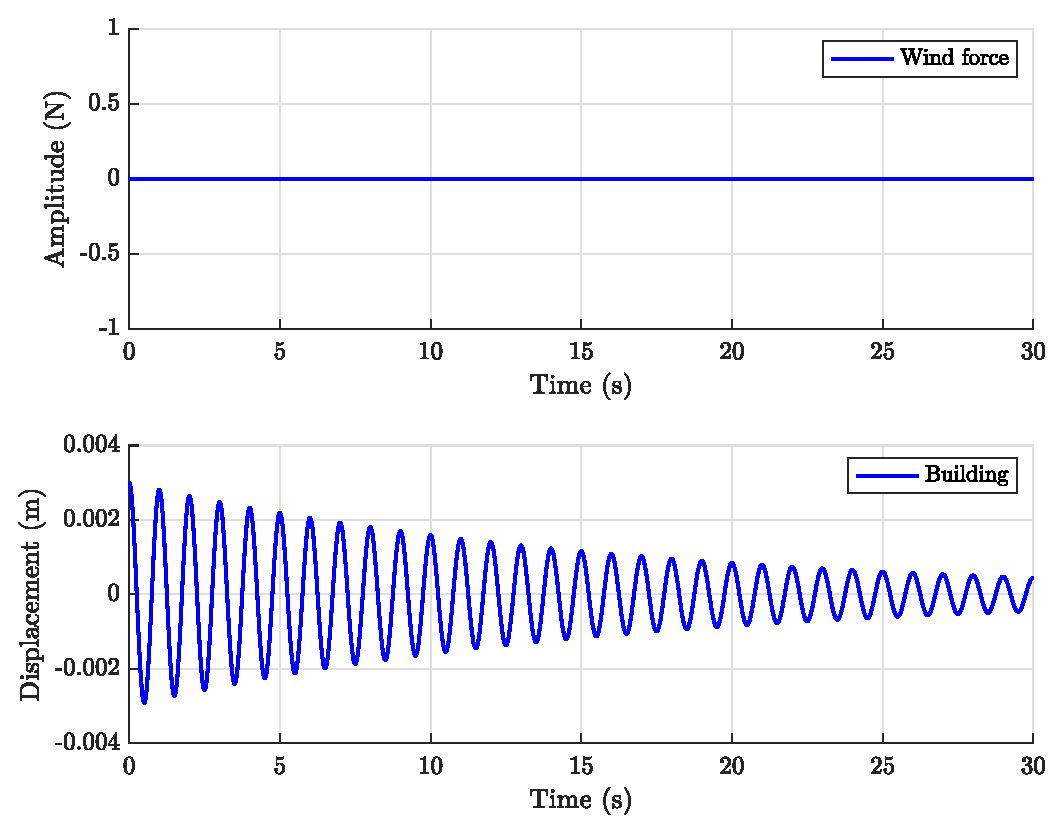
\includegraphics[width=\textwidth]{resources/eps/initial-conditions.eps}
    \caption{Open loop simulation during \SI{30}{\second} with initial conditions}
\end{figure}
We can see that our system is very reactive: the building oscillates quite quickly. He very quickly regains his reference position.

\subsubsection{Constant wind force}
For this simulation, we applied a constant wind with zero initial conditions.
\begin{figure}[H]
    \centering
    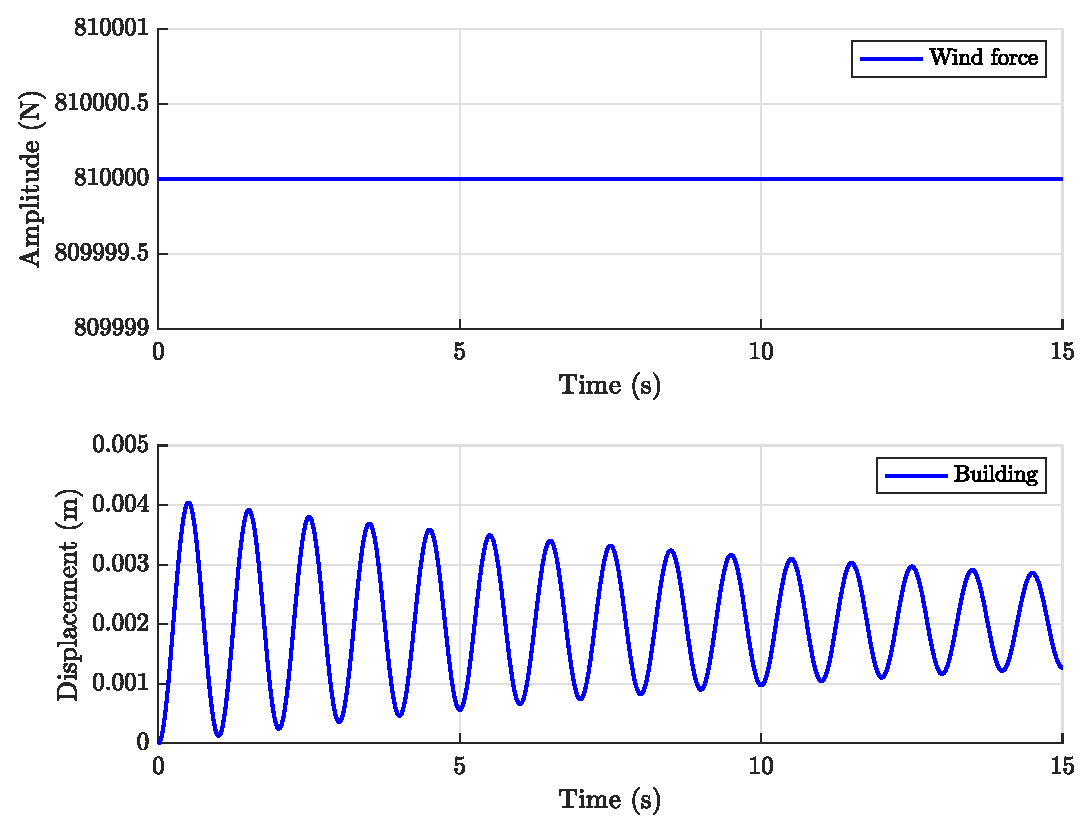
\includegraphics[width=\textwidth]{resources/eps/constant-wind.eps}
    \caption{Open loop simulation during \SI{30}{\second} for a constant wind force}
\end{figure}
In this case, we can see that the building also oscillates very quickly. These oscillations decrease quickly enough over time to finally stabilize at a position slightly different from its reference position.

\subsubsection{Sinusoidal wind force}
For this simulation, we applied a sinusoidal wind with zero initial conditions.
\begin{figure}[H]
    \centering
    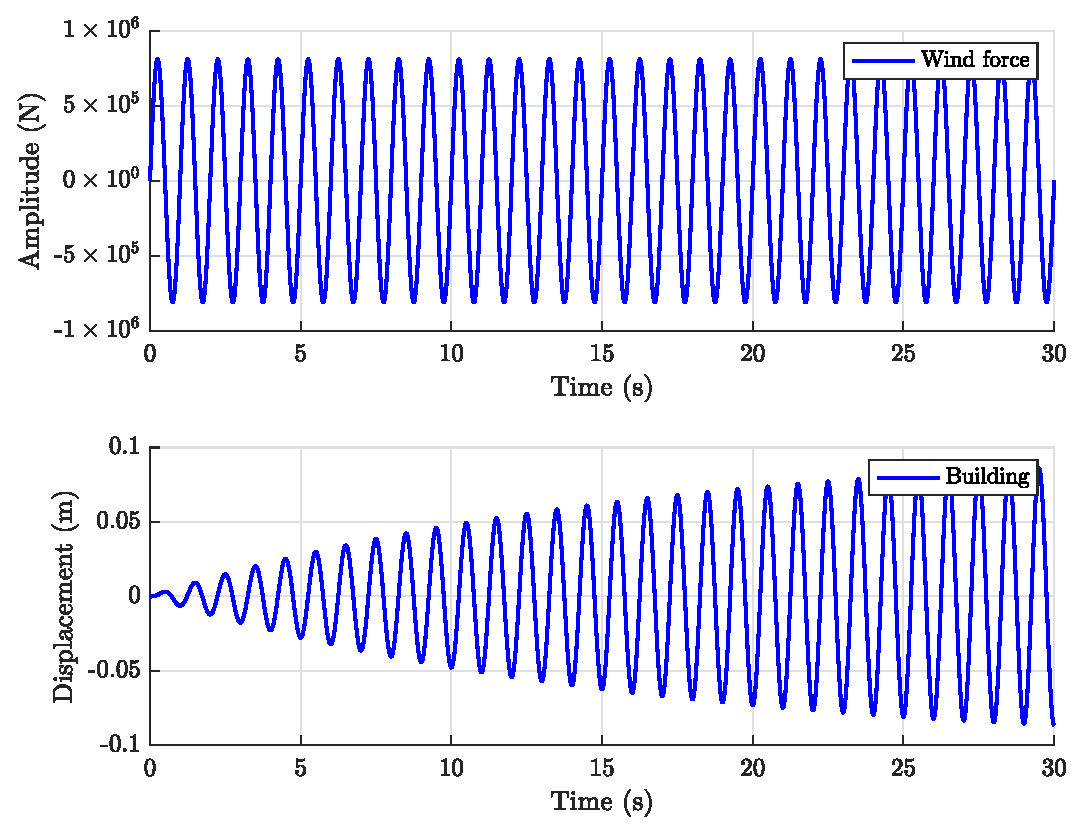
\includegraphics[width=\textwidth]{resources/eps/sinusoidal-wind.eps}
    \caption{Open loop simulation during \SI{30}{\second} for a sinusoidal wind force}
\end{figure}
We can see that the building's oscillations gradually increase, but quite rapidly, over time. A longer simulation has shown that these oscillations stabilize at a maximum value of \SI{0.1}{\meter} after about 30 seconds.

\subsubsection{Random wind force}
For this simulation, we applied a random wind with zero initial conditions.
\begin{figure}[H]
    \centering
    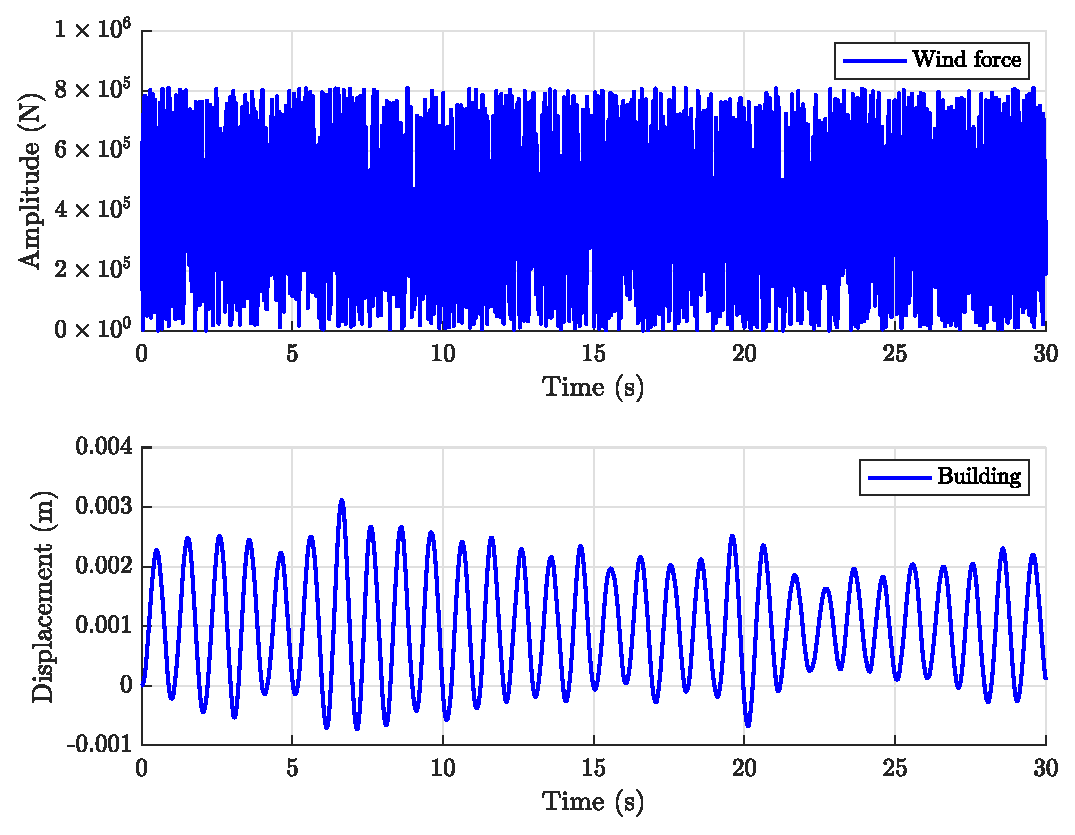
\includegraphics[width=\textwidth]{resources/eps/random-wind.eps}
    \caption{Open loop simulation during \SI{30}{\second} for a random wind force}
\end{figure}
It can be seen that the building oscillates more or less identically and rapidly over time around a position slightly offset from its reference position.

\subsubsection{Relation with the eigenvalues and utility of a controller}
As mentioned in section \ref{sec:eigenvalues}, the eigenvalues of our system suggest that it is very reactive. Indeed, this has been observed on the different simulations : the building oscillates very quickly.\par
Eigenvalues also indicate that the system is stable. Again, this information could be found on the simulations : for a variation in initial conditions, or when the wind force is constant (or decreasing), the system tends to return to its reference position.\par
Although the movements of our building are quite small, a controller could reduce them even more, or even eliminate them completely after a while. Another role of the controller could be to slow down our system so that the building oscillates less quickly.

% Observability
\subsection{Observability}
To determine whether or not the system is observable, one computes the observability matrix thanks to Matlab function (\texttt{obsv}).\par
The matrix is full rank (verified with Matlab), the system is thus fully observable.\par
As seen on the matrix C, one needs one sensor. According to the place of the non zero value, this sensor has to measure the $x_1$ state, namely the horizontal position of the top of the building $d_1$. This state is indeed the objective of the active mass damper and has thus to be observed. The sensor chosen is an accelerometer.

% Controllability
\subsection{Controllability}
To determine whether or not the system is controllable, one computes the controllable matrix thanks to Matlab function (\texttt{ctrb}). In order not to take into account the uncontrollable input (wind), only the second column of the B matrix was kept for the calculation.\par
The matrix is full rank (verified with Matlab), the system is thus fully controllable.\par
As seen on matrix B, one needs only one actuator. The first column of the $B$ matrix represents the wind, while the second one concerns the damper. This latter is indeed the only controllable input and contains two non-zero elements. As a result, only one actuator is needed, and acts on two states, the speed of the building and the speed of the damper, as they take place on $x_2$ and $x_4$. The actuator chosen is a servo motor.
